\documentclass[a4paper]{article}

\usepackage[T1]{fontenc}
\usepackage[utf8]{inputenc}
\usepackage{graphicx}
\usepackage{fixme}

\usepackage[english, french]{babel}

\usepackage{hyperref}

\usepackage[sorting=ynt, maxnames=10, doi=false, url=false]{biblatex}
\addbibresource{biblio.bib}
\AtEveryBibitem{\clearfield{note}}

\usepackage{palatino}

\newcommand{\eg}{{\textit{e.g.~}}}
\newcommand{\etal}{{\textit{et al.~}}}
\newcommand{\ie}{{\textit{i.e.~}}}

\title{Vers une cognition sociale chez les robots \\ 
    {\large Activités scientifiques antérieures et programme de recherche}}

\author{Séverin Lemaignan}
\date{}

%%% Body
\begin{document}
\maketitle

Ce document présente, dans sa première partie, l'ensemble de mes travaux de
recherche, organisés par grands axes, puis, dans sa seconde partie, mon projet
de programme de recherche.

\section{Activités de recherche antérieures}
\newrefsection

Ma première contribution à une conférence internationale remonte à 2006, lorsque
j'étais étudiant en master à l'ENSAM/ParisTech. Cet article formalisait une
ontologie pour décrire les processus industriels, et étudiait comment elle
pouvait être appliquée à l'automatisation des lignes de production, via un
paradigme multi-agent~\cite{lemaignan2006mason}. Depuis cette période, mes
activités de recherche se sont focalisées sur cette question: quels ponts bâtir
entre intelligence artificielle (et en particulier, les techniques de
l'ingénierie des connaissances) et interaction homme-robot.

Je propose de présenter ces travaux suivant trois axes : mon travail sur les
outils sémantiques pour la robotique, puis mes recherches sur les liens entre
connaissance et interaction située, puis enfin mes contributions plus récentes
sur la question de la cognition en robotique dans le contexte de l'interaction.

Je terminerai cette première partie en présentant mes autres activités de
support scientifique (enseignement, organisation de colloques et de rencontres
scientifiques, développement logiciels notables).

Toutes les références bibliographiques mentionnées dans cette première partie
sont par ailleurs des références vers des publications dont je suis auteur ou
co-auteur.

\subsection{Outils sémantiques pour la robotique%
  \label{semantic-tools-for-robotics}%
}

Le point de départ de mes recherches se situe dans l'application de techniques
sémantiques à la robotique. J'ai initialement été introduit aux outils de
l'ingénierie des connaissances durant mon master recherche à l'université Paris
5, que je menais en parallèle de ma formation d'ingénieur à l'ENSAM/ParisTech et
au Karslruhe Institute of Technology (KIT). Mon projet de fin d'étude s'est
intéressé à l'utilisation des ontologies pour le contrôle de systèmes
multi-agents dans un contexte industriel, et a débouché sur une première
publication~\cite{lemaignan2006mason}, depuis citée plus de 80 fois.

J'ai ensuite rejoint pendant un an l'INRIA en tant qu'ingénieur de recherche,
sous la supervision de Michel Parent.  J'ai continué d'y développer, de manière
concrète, l'utilisation d'ontologies pour la robotique, en proposant une
architecture de contrôle de véhicules autonomes basée sur un réseau d'ontologies
dynamiques et partagées entre robots~\cite{mehani2007networking}.

Ces deux premières expériences ont formé le point de départ de mon travail de
doctorat au LAAS-CNRS (2008-2012), sous la supervision de Rachid Alami. La
problématique initiale qui se posait alors était la suivante : les robots
d'interaction développés dans le laboratoire manipulent des états internes
complexes et dynamiques, mais difficilement observables. L'intuition poussait à
croire qu'en rendant \emph{explicites} les flux de connaissances entre
composants logiciels du robot, non seulement le comportement du robot serait
plus facile à interpréter, mais de plus, de nouvelles opportunités s'ouvriraient
pour les tâches décisionnelles du robot, comme la planification symbolique ou la
supervision du robot.

J'ai donc proposé de concevoir un ``tableau noir'' sémantique à travers lequel
les différents modules décisionnels du robot communiquent, en échangeant des
messages dont la sémantique est explicite. Ce projet, \emph{OpenRobots
Ontology}, est une des contributions importante de mon
doctorat~\cite{Lemaignan2010}, et représente le fil rouge des projets
que j'ai menés par la suite.

Je présente dans~\cite{lemaignan2013explicit} les principales leçons tirées du
déploiement d'une base de connaissances active comme \emph{OpenRobots Ontology}
dans des architectures robotiques complexes (près de 70 modules logiciels
fonctionnant en parallèle lors des expériences menées avec le robot PR2). L'idée
de définir les composants du robot en terme d'interfaces sémantiques (les
connaissances dont il a besoin d'une part, et les connaissances qu'il produit
d'autre part) apparait comme un apport important, de même que le principe
d'utiliser les ontologies pour générer l'ensemble des inférences
\emph{triviales} (du type ``tous les enfants sont aussi des humains''),
essentielles pour que le robot puisse raisonner et interagir dans un référentiel
de connaissances partagé avec l'homme.

Un autre intérêt de cette classe d'outils sémantiques est l'acquisition
automatique et l'intégration par le robot de connaissances issues du web
sémantique. Le projet \emph{OpenRobots Ontology} s'appuie déjà sur des
standards comme {\sc OpenCYC}, et j'ai eu l'occasion d'être invité durant la
conférence INNOROBO 2013 à présenter les pistes permettant d'approfondir les
interactions entre outils sémantiques et robotique.

\subsection{Connaissances et interaction située%
  \label{semantic-tools-for-grounded-interaction}%
}

Au-delà des recherches sur les outils sémantiques eux-mêmes, mon doctorat visait à
explorer l'intérêt d'une approche sémantique pour l'interaction située, ce qui
inclut les questions d'ancrage symbolique (\emph{symbol grounding}), de
communication, de traduction d'un modèle symbolique en actions, de
représentation des agents interagissant, et en particulier, de la représentation
de leur croyances et intentions.

L'acquisition d'un modèle symbolique du monde et la capacité du robot à prendre
le point de vue des autres agents (\emph{prise de perspective}) a été un des
premiers résultats important~\cite{Lemaignan2011}.  L'utilisation d'une base de
connaissance symbolique permet de représenter le modèle des croyances de chacun
des agents, et ouvre des applications comme l'identification automatique des
propriétés discriminantes des objets de l'environnement du point de vue de
chaque agent~\cite{ros2010which} (\emph{Best Paper Award}, RoMAN 2010).

Un autre domaine pour lequel l'introduction de flux de connaissances explicites
a été particulièrement fructueuse est celui de la communication naturelle,
située et multi-modale. Parce que le robot manipule en interne des concepts dont
la sémantique est définie et non ambigüe, j'ai montré qu'il est possible alors
d'analyser et de donner du sens à une gamme étendue d'interactions verbales en
langue naturelle~\cite{Ros2010a, lemaignan2011dialogue, lemaignan2013talking}.
J'ai aussi montré que l'intégration d'autres modalités de communication (comme
les gestes) devient transparente, du fait que tous les modules du robot
produisent des connaissances déjà articulées les unes aux autres à travers une
même ontologie générale~\cite{lemaignan2011what, Lemaignan2011a}.

La couche d'abstraction sémantique que j'ai proposé à enfin ouvert un certain
nombre d'opportunités dans le domaine des actions conjointes homme-robot. Parce
que les croyances, non seulement du robot, mais aussi des agents avec lesquels
le robot interagit, sont représentées de manière explicite, le planificateur
symbolique de tâches peut générer des plans d'action
conjoints~\cite{alami2011when, Lemaignan2012, clodic2013on}. De même, en
maintenant à jour le modèle des croyances de l'homme, il est possible d'influer
de manière symbolique sur l'exécution de ces actions
conjointes~\cite{gharbi2013natural}.

Ces possibilités ont été illustrées dans une série d'expériences menées dans le
cadre du projet européen CHRIS, et dans lesquelles le robot construit un modèle de
l'homme au fil de l'interaction, et l'exploite pour adapter son comportement durant
des séquences de jeu, incluant des inversions de rôle~\cite{Lallee2010b,
Lallee2011, Lallee2012}.



\subsection{Cognition pour l'interaction%
  \label{cognition-for-interaction}%
}

Le travail que j'ai mené sur la représentation et la manipulation de la
connaissance pour l'interaction située a débordé de son périmètre
initial pour s'élargir à la question plus générale de la \emph{cognition pour
l'interaction} chez les robots.

Ce champ de recherche est vaste, et est au c\oe ur du projet de recherche que je
présente dans la seconde partie de ce dossier.

J'ai travaillé sur cette question sous deux angles : une perspective
intégrative d'une part, et une perspective plus exploratoire d'autre part.

J'ai ainsi coordonné l'écriture de deux articles de journaux et d'un chapitre de
livre s'intéressant à l'architecture cognitive du robot dans sa
globalité~\cite{alami2011when, Lemaignan2012, lemaignan2014human}. Ils
présentent en particulier comment la manipulation explicite de connaissances
symboliques ouvre des voies nouvelles pour l'intégration des multiples processus
décisionnels au sein d'une architecture robotique complexe.

Dans~\cite{lemaignan2014human}, je présente en particulier les
principaux défis que l'interaction homme-robot pose à l'intelligence
artificielle, en termes d'ancrage, de modèles mentaux, d'attention et
d'action conjointe, d'interaction naturelle multi-modale ou encore d'analyse
spatiale, temporelle et contextualisée de situation. Je montre que ces
questions peuvent être en partie abordées de manière holistique, en s'appuyant
sur des interfaces sémantiques clairement définies.

Parallèlement à cet effort de synthèse au niveau de l'architecture du
robot, j'ai mené plusieurs expériences centrées sur des aspects cognitifs
précis. Ainsi, les expériences de \emph{False Beliefs}~\cite{warnier2012when},
liées à la mise en place d'une théorie de l'esprit chez le robot.

Ainsi aussi, le travail que j'ai mené durant mon post-doctorat au LAAS-CNRS
(2012-2013) sur les besoins spécifiques de représentation pour l'interaction.
L'objectif était de concevoir une technique de représentation fusionnant le
\emph{Umwelt} (\emph{monde propre}) spatial et temporel du robot en un modèle
amodal pouvant servir de point d'entrée pour les fonctions cognitives
supérieures du robot. Le prototype que j'ai développé est construit autour de
l'idée de \emph{mondes} que le robot peut manipuler en fonction de son contexte
et de ses besoins.  Chaque monde combine une représentation géométrique et une
\emph{histoire} dans laquelle il peut librement naviguer. Les différents mondes
peuvent évoluer indépendamment, et on peut alors les concevoir comme des mondes
hypothétiques, adaptés par exemple pour simuler et représenter le résultat d'une
planification.

Par ailleurs, je me suis intéressé à la question de la cognition pour
l'interaction sous l'angle complémentaire des mécanismes cognitifs
\emph{humains} en jeu durant une interaction.

J'ai commencé à m'intéresser à cet aspect dans le cadre de la robotique
pédagogique. D'abord de manière expérimentale au sein de l'association Planète
Sciences~\cite{stinckwich2007squeakbot}, puis de manière plus théorique en
suivant un master recherche à l'Université Paris 5 dans le domaine des
Environnements Informatiques pour l'Apprentissage Humain (EIAH), ce qui n'a permis
d'acquérir un certain nombre de bases en interaction homme-machine (HCI), en
particulier en ergonomie.

Ces deux premières expériences ont guidé le choix de mon post-doctorat à l'École
Polytechnique Fédérale de Lausanne (2013-...), où j'ai pris en charge la
coordination des activités robotiques au sein du laboratoire d'ergonomie
éducative. Ce laboratoire (CHILI-EPFL) est connu pour son expertise dans l'étude
des interactions homme-machine et homme-homme durant les phases d'apprentissage.
J'y ai acquis le savoir-faire nécessaire à la menée et l'analyse d'expériences
in-situ (écologiquement valides) impliquant des sujets humains.

J'y supervise deux projets principaux. Le premier s'intéresse aux interactions
sur la durée entre un robot et des enfants~\cite{fink2014which}. Il m'a
permis, entre autres, d'étudier l'impact des comportements anthropomorphiques
sur l'interaction homme-robot sur le long terme~\cite{lemaignan2014dynamics}. Le
second projet repose sur l'idée du \emph{learning by teaching}, et propose de
mettre en place une interaction enfant-robot durant laquelle l'enfant
\emph{montre} au robot (Nao) comment écrire. La question est de savoir si
une telle situation peut créer une forme d'interaction originale qui permette
d'établir une relation pérenne et qui soutienne efficacement l'apprentissage.

\subsection{Autres activités de support scientifique}

Dans cette dernière section, je propose de parcourir brièvement mes autres
activités scientifiques, afin d'inscrire ma candidature dans le cadre plus large
de l'animation de la vie scientifique.

\subsubsection{Enseignement et encadrement}

Depuis mon entrée dans la recherche à l'INRIA en 2006, j'ai développé une
activité d'enseignement en parallèle de mon travail de recherche.

J'ai été ainsi assistant d'enseignement en mécatronique à Mines ParisTech
pendant un an (sous la supervision de Bruno Steux), puis, durant mon doctorat,
j'ai été moniteur à l'INSA Toulouse, impliqué en particulier sur les travaux
dirigés et pratiques en Prolog, sur les ontologies, en Java, ADA et SQL.

J'ai aussi organisé et animé de nombreux cours et ateliers dans plusieurs
domaines de la robotique et du développement logiciel. Je suis ainsi intervenu
sur la programmation en robotique avec ROS (\emph{Robot Operating System}), les
techniques de développement collaboratif, les cycles de développement ou encore
l'utilisation d'outils sémantiques comme les ontologies. J'ai organisé plusieurs
tutoriels internationaux sur la simulation en robotique (comme lors de la
conférence EURON, en 2012 au Danemark), et je suis, depuis 2005, formateur au
sein de l'association \emph{Planète Sciences} sur toutes les questions de
robotique pédagogique.

Par ailleurs, j'ai été amené à encadrer plusieurs étudiants ces dernières
années. Une dizaine d'étudiants au niveau master au total (dont le travail, pour
certains, a débouché sur des publications, comme~\cite{Lemaignan2011a}),
et, durant mon post-doctorat à l'EPFL, deux doctorants (Julia Fink et Shruti
Chandra). L'une travaille sur la question de l'anthropomorphisme lors
l'interaction homme-machine de longue durée, tandis que l'autre travaille sur
l'utilisation de robots compagnons pour soutenir les enfants en difficulté face
à l'apprentissage de l'écriture.

\subsubsection{Associations scientifiques et dissémination}

Outre mon implication, déjà mentionnée, dans l'association de diffusion de la
culture scientifique \emph{Planète Sciences}, dont j'ai présidé pendant deux ans
la section robotique, j'ai été, durant mon doctorat, vice-président de
l'association \emph{InCOGnu}, antenne Sud-Ouest de la Fédération Française des
Étudiants et Jeunes Chercheurs en Sciences de la Cognition (FRESCO). Mon
activité au sein de cette association m'a permis de m'ouvrir à la dimension
interdisciplinaire de la recherche en sciences cognitives, en particulier à
travers les conférences mensuelles que nous avons proposés, et où intervenait
des chercheurs confirmés issus de tous les domaines des sciences cognitives.
C'est aussi dans le cadre d'InCOGnu que j'ai participé à l'organisation de la
conférence nationale CJCSC à Toulouse en 2009.

Plus récemment, j'ai organisé et animé en 2012 le premier workshop international
sur le simulateur MORSE auquel une quinzaine de chercheurs européens ont participé.

Je suis par ailleurs relecteur régulier pour les principales conférences en
robotique (IROS, ICRA, RoMAN, HRI).

Parmi les actions que j'ai mené à destination du grand public, la pièce de
théâtre Roboscopie~\cite{lemaignan2012roboscopie} peut être mentionné : à l'automne
2011, j'ai mis en place, en collaboration avec un metteur en scène et un
comédien professionnel, une pièce de théâtre d'une vingtaine de minutes dans
laquelle un robot PR2 donne la réplique à un homme. La pièce interroge sur un
mode métaphorique comment hommes et robots peuvent trouver un espace de vie et
de compréhension mutuels. La pièce a été présentée devant environ 400 personnes
durant le festival La Novela 2011, à Toulouse.

\subsubsection{Contributions logicielles notables}

Au-delà des développements logiciels directement en lien avec mon travail de
doctorat, et précédemment mentionnés (\emph{OpenRobots
Ontology}~\cite{Lemaignan2010} et le module d'analyse de la langue naturelle
{\sc Dialogs}~\cite{Lemaignan2011a}), je me suis impliqué dans le développement
de plusieurs autres projets significatifs dans la communauté robotique.

Le premier de ces projets est le simulateur MORSE~\cite{Echeverria2011,
echeverria2012simulating}. Le projet a pris une ampleur certaine, avec plus de
25 contributeurs du monde entier, son intégration officielle dans le projet
Debian, et un workshop annuel. J'en suis le concepteur initial, l'un des
principaux contributeurs, et j'anime la communauté des développeurs. J'ai en
particulier travaillé sur l'utilisation de MORSE en interactions
homme-robot~\cite{lemaignan2012morse}.

ROS est un autre projet dans lequel je suis impliqué.  J'ai plusieurs
contributions au niveau noyau, et je fais partie de l'équipe qui a adapté ROS
pour le robot Nao.

Enfin, je suis impliqué dans la conception d'outils logiciels plus spécialisés,
comme GenoM~\cite{mallet2010genom3}.

\subsection{Pour conclure}

Pour conclure cette première partie, je souhaite souligner trois traits de mon
parcours : la place particulière donnée à la validation expérimentale de mes
recherches, la dimension internationale de mon itinéraire, et l'importance de
l'interdisciplinarité.

La table~\ref{experiences} liste les principales expériences que j'ai menées
durant ces dernières années. Comme souvent en robotique, elles sont le résultat
d'un travail d'équipe, mais j'en ai été, pour chacune d'elles, un des
principaux instigateurs.

À l'exception de l'expérience \emph{CoWriter 1}, récente, toutes ces expériences
ont débouché sur des publications, et, ensemble, illustrent la place que
j'accorde à la validation expérimentale de mes recherches. Ces expériences ont
été réalisées sur des robots (et non en simulation), et incluent aussi des
études centrées sur les comportements humains en présence de robots
(\emph{Roboscopie}, \emph{CoWriter}, \emph{Ranger}).

\begin{table*}
\begin{center}

    \begin{tabular}{lp{6cm}l}
\bf{Expérience} & Focus & Ref. \\
\hline
{\it Point \& Learn} (2010) & Acquisition interactive de connaissances & \cite{Lemaignan2010} \\
{\it Spy Game} (2010) & Discrimination interactive d'objets & \cite{ros2010which} \\
{\it Moving to London} (2011) & Interaction multi-modale, \newline prise de perspective & \cite{lemaignan2011what} \\
{\it Roboscopie} (2011) & Théâtre, \newline réflexion sur le futur de la HRI & \cite{lemaignan2012roboscopie} \\
{\it Cleaning the table} (2011) & Intégration complète & \cite{alami2011when} \\
{\it I'm in your shoes} (2012) & Fausses croyances & \cite{warnier2012when} \\
{\it Give me this} (2012) & Manipulation naturelle conjointe & \cite{gharbi2013natural} \\
{\it Aperitif time} (2012) & Interaction multi-modale, \newline prise de perspective & \cite{lemaignan2013talking} \\
{\it CoWriter 1} (2013) & \emph{Expérience enfant-enfant}, \newline protocoles
d'interaction, expérience de terrain &  \\
{\it Ranger} (2013) & Expérience enfant-robot, \newline projections cognitives en HRI &
\cite{fink2014which, lemaignan2014dynamics} \\
\hline

\end{tabular}
\end{center}
\caption{Principales expériences menées en interaction homme-robot.}
\label{experiences}
\end{table*}


Le deuxième aspect particulier de mon parcours de jeune chercheur est sa
composante internationale. Dès la période du master, j'ai fait le choix de
suivre un cursus d'ingénieur franco-allemand, qui m'a conduit près de deux ans
en Allemagne, au Karlsruhe Institute of Technology (KIT), et m'a finalement
permis d'obtenir en 2006 la médaille d'or de l'ENSAM/ParisTech. J'ai aussi,
pendant ce master, mené pendant six mois des travaux de recherche en physique
fondamentale au Paul Scherrer Institute en Suisse, ce qui a représenté ma
première immersion à proprement parler dans le monde académique international.

Suite à cela, et bien que cela ne fasse pas partie de mon parcours de chercheur
proprement dit, j'ai voyagé pendant une année autour du monde (2007-2008),
expérience importante tant au niveau personnel qu'au regard de mon ouverture à
l'international.

J'ai souhaité ensuite organiser mon doctorat en co-tutelle, cette
fois avec la Technische Universität de Munich (TUM), ce qui m'a conduit à
nouveau à séjourner plusieurs mois en Allemagne. Mon doctorat allemand, noté, a
reçu la meilleure appréciation possible (\emph{Cum Suma Laude}) dans le système
allemand.

Enfin, le post-doctorat que je réalise actuellement à l'École Polytechnique
Fédérale de Lausanne (EPFL) est la plus récente escale internationale de mon
parcours.

Cet itinéraire international reflète la diversité des environnements
intellectuels dans lesquels j'ai évolué, et me permet aujourd'hui de bien
appréhender le tissu scientifique européen, en particulier dans le domaine de la
robotique cognitive.

Le troisième aspect particulier de mon parcours est sa dimension
interdisciplinaire : depuis la période du master, durant laquelle j'ai suivi en
parallèle une formation d'ingénieur et une formation universitaire dans le
domaine de l'intelligence artificielle appliquée à l'éducation, j'ai tenté de
garder une ouverture sur les questions de cognition humaine. C'est ainsi que je
me suis impliqué dans l'association des jeunes chercheurs en sciences
cognitives, c'est ainsi aussi que j'ai choisi de rejoindre en post-doctorat un
laboratoire centré sur les technologies pour l'éducation, avec un savoir-faire
fort dans le domaine de l'expérimentation homme-machine. J'y ai acquis une
expérience essentielle pour pouvoir aujourd'hui mener des expériences en
interaction homme-robot qui soient pertinentes, écologiquement valides, et
méthodologiquement rigoureuses.

\printbibliography
\clearpage

%%%%%%%%%%%%%%%%%%%%%%%%%%%%%%%%%%%%%%%%%%%%%%%%%%%%%%%%%%%%%%%%%%%%%%%%%%%%%%%%%%%%%%%%%%%%%%%%%%%%%%%
%%%%%%%%%%%%%%%%%%%%%%%%%%%%%%%%%%%%%%%%%%%%%%%%%%%%%%%%%%%%%%%%%%%%%%%%%%%%%%%%%%%%%%%%%%%%%%%%%%%%%%%
%%%%%%%%%%%%%%%%%%%%%%%%%%%%%%%%%%%%%%%%%%%%%%%%%%%%%%%%%%%%%%%%%%%%%%%%%%%%%%%%%%%%%%%%%%%%%%%%%%%%%%%

\section{Projet de programme de recherche}
\newrefsection

La présentation de mes activités de recherche antérieures peut être comprise comme
autant de regards sur la problématique de la cognition sociale chez les robots : la
question pratique de la représentation et de la manipulation des connaissances,
la question des pré-requis sémantiques de l'interaction naturelle (verbale en
particulier), la question de la cohérence et de la faisabilité d'une
architecture cognitive intégrée pour la robotique d'interaction, la question,
aussi, de l'évaluation de l'engagement homme-robot sur le long terme.

Ces différentes facettes sont les pièces d'un puzzle auquel je me propose de
travailler dans sa globalité : \textbf{comment comprendre l'idée de \emph{cognition
sociale} chez le robot, comment la construire, comment l'évaluer ?}

Ce projet s'articule en plusieurs axes, que j'expose plus en détail ci-après.
La première question que je souhaite poser est celle-ci : Que nous enseignent
les sciences cognitives \emph{humaines} en terme de compétences cognitives
nécessaires à l'interaction entre agents et en terme d'évaluation de ces
compétences ? Une synthèse des travaux existants en sciences humaines et
neuro-sciences cognitives, et l'important travail d'adaptation à la robotique
qui en découle, apparaissent aujourd'hui incontournables pour progresser sur les
questions d'interaction sociale entre hommes et robots.

La question théorique sous-jacente est celle de la compréhension, de la
définition et de l'application de l'idée de cognition sociale en robotique. Je
souhaite donner corps à cette problématique, aujourd'hui floue car
multi-factorielle, en re-pensant l'existant (les (neuro-)sciences cognitives, donc,
mais aussi les architectures cognitives telle qu'on les connait en intelligence
artificielle) dans le cadre de la robotique sociale, avec ses dimensions
particulières (relations interpersonnelles, incarnation, sous-spécification,
dynamique). Il s'agit non seulement de construire l'idée de cognition sociale
chez le robot, mais aussi de l'envisager de manière concrète, en terme
d'implémentation sur des robots.

Un aspect saillant de cette question, et dont je propose de faire un autre de
mes axes de recherche, est la question de la \emph{représentation} de
l'environnement spatial, temporel, social et contextuel du robot. La littérature
s'intéresse essentiellement aux deux premiers points. Il me semble que les deux
derniers sont des objets encore peu étudiés et pourtant essentiels pour une
prise de décision autonome et complexe en interaction homme-robot.

Enfin, je souhaite inscrire ce programme de recherche dans une perspective
expérimentale forte. La menée systématique d'expériences d'interaction en
milieux écologiquement valides reste rare et sujette à des faiblesses
méthodologiques. En m'appuyant sur l'expérience que j'ai acquise en
post-doctorat, je souhaite en particulier travailler à la mise en place d'un
référentiel expérimental pour l'évaluation cognitive des robots, qui serait
aisément reproductible dont la méthodologie serait rigoureusement validée.

Ce projet de programme de recherche mêle étroitement robots et humains. Bien que
mise en avant de manière répétée dans les orientations scientifiques européennes
(voir par exemple la place qu'y consacre l'agenda Horizon2020 dans la section
\emph{Future and Emerging Technologies}), la robotique cognitive d'interaction
est relativement peu représentée dans le paysage scientifique français. Au sein
du CNRS, les trois principaux laboratoires travaillant sur cette thématique sont
l'\emph{Institut des Systèmes Intelligents et de Robotique} (ISIR) à Paris, le
\emph{Laboratoire d'Analyse et d'Architecture des Systèmes} (LAAS) à Toulouse,
et le \emph{Robot Cognition Laboratory} (RLC) à Lyon (unité mixte INSERM). Le
LAAS et le RLC sont des laboratoires avec lesquels j'ai déjà travaillé, et qui
seraient tout à fait adaptés pour y développer mes thèmes de recherche ; je
souhaiterais cependant, en premier choix, rejoindre l'ISIR : ce laboratoire a
une expertise reconnue aussi bien en cognition artificielle (avec de nombreuses
collaborations interdisciplinaires), que sur les questions d'interaction
(notamment au niveau du traitement des signaux sociaux). L'ISIR a récemment
acquis un robot PR2, prenant ainsi la direction de recherches sur des
architectures décisionnelles intégrées. Mon expérience antérieure avec ce type
d'architecture et le projet que je propose ici s'inscrivent naturellement dans
cette dynamique.

\subsection{Axe 1 -- Définir la cognition sociale chez le robot}

Comme je l'ai présenté dans~\cite{lemaignan2014human}, si la robotique
cognitive, qui hérite à ce titre de la psychologie cognitive, s'intéresse aux
processus mentaux comme l'\emph{attention}, l'utilisation du \emph{langage}, la
\emph{mémoire} ou les processus de \emph{prise de décision}, la cognition
sociale y ajoute les aspects lié à la prise en compte des interactions avec
d'autres agents : \emph{représentation des croyances}, \emph{prise de
perspective}, \emph{action conjointe}, et tous les aspects liés à la
\emph{communication}.

L'une des difficultés importantes à laquelle la communauté fait face est
l'absence de référentiel permettant d'évaluer, et donc de comparer et de mesurer
les progrès des capacités cognitives des robots.  Cela tient à deux raisons
principales : d'une part, le périmètre exact de ce qu'on appelle la robotique
cognitive est relativement mal défini, ce qui rend difficile la création d'une
mesure synthétique des capacités cognitives ; d'autre part, la plupart des
outils d'évaluation à notre disposition viennent de l'étude de la cognition
humaine, et sont concrètement souvent difficile à appliquer aux robots car la
hiérarchie des compétences cognitives chez les robots est différente de celle de
l'homme : les compétences langagières, par exemple, sont difficilement
comparable. La production verbale, essentiellement traitée par la synthèse
vocale, est considérée pour un robot comme un problème moins difficile que la
compréhension orale (qui requiert, outre la reconnaissance vocale, une analyse
syntaxique et sémantique généralement difficile). Or les tests de langage que
l'on rencontre en psychologie cognitive vont typiquement se focaliser sur la
capacité à parler, en faisant l'hypothèse que l'enfant comprend ce qu'on lui dit.

De fait, la communauté robotique s'appuie aujourd'hui essentiellement sur des
évaluations qualitatives. Langley~\etal\cite{Langley2006} suggère ainsi cinq
dimensions d'évaluation : la \emph{généralité} du système (peut-il s'adapter à
une nouvelle tâche?), la \emph{rationalité} ou pertinence des
inférences/raisonnements/décisions que le système prend, la \emph{réactivité} et
la \emph{persistance} qui évalue si le comportement du système est approprié en
cas de changements non-anticipés, la capacité du système à \emph{améliorer sa
performance} comme fonction des connaissances supplémentaires qu'on lui fournit,
et enfin, \emph{l'autonomie} du système. Ces dimensions sont cependant
générales, et peu opérationnelles.

Un certain nombre d'outils issus de la psychologie cognitive ont déjà été
explorés de manière concrète sur des robots, comme les expériences d'inversion
de rôle~\cite{Lallee2010b}, de fausses croyances (\emph{False
Beliefs}~\cite{Leslie2000}), liées à la théorie de l'esprit~\cite{Breazeal2006,
warnier2012when, trafton2013act}, ou encore le \emph{Token
test}~\cite{DiSimoni1978} pour l'évaluation de certaines compétences
linguistiques~\cite{Mavridis2006}. Ces expériences ont montré qu'il était
possible et utile de ré-utiliser en les adaptant des tests de psychologie
cognitive en robotique. Elles restent cependant ponctuelles, et un travail plus
systématique et plus global reste à faire. D'autant plus que, comme l'ont
récemment souligné Zhang~\etal\cite{zhang2013evaluation}, les environnements et
métriques existants pour l'évaluation des performances cognitives des robots se
focalisent pour la plupart sur des capacités physiques, et ne requièrent pas de
capacités avancées de représentation et manipulation de connaissance, sans même
parler de compétences cognitives \emph{sociales}.

%Eux-même proposent leur une métrique basée sur la mesure du \emph{Fitness to
%Ideal Model} (FIM) d'un comportement, qu'ils corrèlent à la \emph{longueur de
%description} (DLen) de la commande qui a déclenchée le comportement. L'hypothèse
%étant que, pour un comportement donné, plus le robot a des capacités cognitives
%avancées, plus courte (c'est à dire, sous-spécifiée) pourra être la commande, le
%robot inférant le reste. Cette piste est intéressante, et est à mettre en
%relation avec d'autres approches issues des sciences cognitives humaines.

Mon objectif est ici de rechercher et de construire un référentiel rigoureux et
opérationnel pour l'évaluation des compétences cognitives des robots, en
s'intéressant à la fois à l'évaluation de chaque capacité cognitive
indépendante, et à la fois à des métriques globales de l'activité cognitive du
robot (dans~\cite{lemaignan2013explicit}, je propose une piste à explorer à ce
sujet en définissant la notion de \emph{charge cognitive} du robot en terme de
flux de connaissances échangés).

Ce premier axe de recherche propose donc de réaliser d'abord la synthèse des
travaux en sciences cognitives aussi bien en terme de construction de
l'interaction que d'évaluation des compétences cognitives, puis ensuite
d'aligner ces résultats avec les spécificités de la robotique. Les objectifs
sont d'une part une définition effective du concept de cognition sociale en
robotique, et d'autre part la conception et l'implémentation d'un référentiel
expérimental d'évaluation des compétences cognitives des robots d'interaction.

\subsection{Axe 2 -- Représentation du monde et cognition}

\begin{figure}
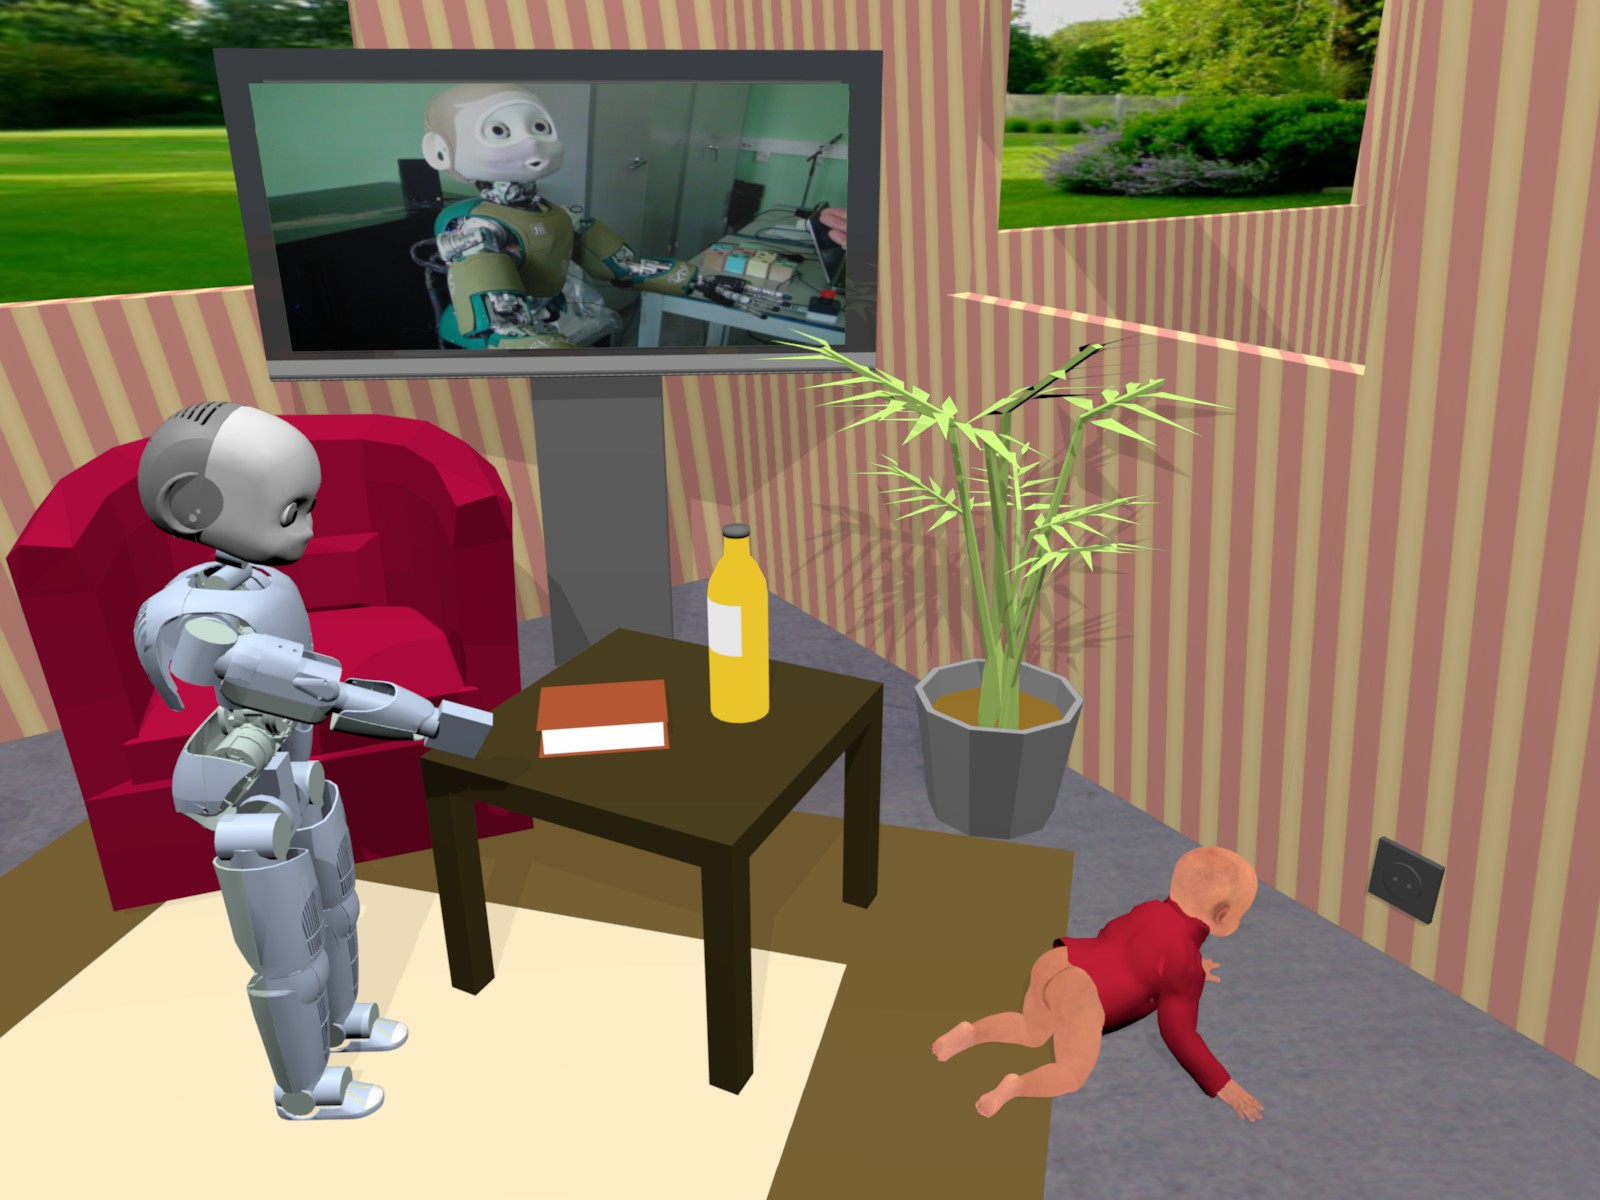
\includegraphics[width=\textwidth]{figs/robots_home_baby_socket.jpg}
\caption{Pour comprendre cette situation et anticiper le danger, il est
    nécessaire de construire une représentation \emph{unifiée} de
    l'environnement, incluant modèle géométrique (l'agencement de la pièce), modèle
    symbolique (le bébé, la prise), modèle temporel prédictif (déplacement du
    bébé), modèle des affordances \emph{pour le bébé} et enfin modèle des
    croyances et intentions du bébé.}
\label{babyplug}
\end{figure}

Le travail que j'ai mené durant mon doctorat m'a amené à analyser huit systèmes
de représentation des connaissances effectivement déployés sur des robots. Un
point clé de comparaison de ces systèmes est leur approche de l'ancrage
symbolique (\emph{symbol grounding}) dans leur environnement physique, et il en
ressort que la capacité pour un robot à représenter son environnement est à la
fois la pierre angulaire de ses capacités cognitives supérieures (raisonnement,
prise de décision, communication) et un défi qui n'est pas aujourd'hui traité
dans toute son ampleur.

Les recherches actuelles sont essentiellement focalisées sur la représentation
géométrique de l'environnement du robot. La construction en ligne de
cartes sémantiques~\cite{Nuechter2008, Galindo2008,
Blodow2011} ou l'utilisation d'affordances fonctionnelles~\cite{Varadarajan2011}
sont des exemples de l'état de l'art au regard de la construction de liens
géométrique-symbolique sur l'environnement spatial du robot.

De même, le travail sur une représentation \emph{amodale} de
l'environnement~\cite{Mavridis2006}, prenant en compte les incertitudes et
permettant de représenter des entités spatiales non-vues (donc de les imaginer),
apporte plusieurs idées importantes, mais se cantonne essentiellement aux
aspects spatiaux.

La représentation de l'environnement temporel du robot a aussi fait l'objet de
recherches (avec les idées de \emph{chroniques}~\cite{Ghallab1996}, les
approches par \emph{fluents}~\cite{mosenlechner2010becoming}, ou encore les
\emph{instantanés} proposés par Mavridis~\cite{Mavridis2006}), mais la plupart
de ces travaux s'apparentent à une journalisation des événements, accompagnée
d'outils d'analyse et d'apprentissage (en général hors-ligne). Ni la possibilité
de naviguer naturellement dans les états antérieurs, ni la création et la
représentation d'états futurs hypothétiques ne sont intégrées au niveau d'une
représentation globale de l'environnement du robot.

Quant à l'intégration de la représentation d'affordances, de contextes (en
particulier, de contextes sociaux, comme dans la figure~\ref{babyplug}, où le
robot est dans un contexte du type ``veiller sur le bébé''), de modèles de
croyances et d'intentions, le travail reste largement à faire (on peut toutefois
mentionner la représentation de différentes perspectives, comme
dans~\cite{ros2010which}). Le premier de ces défis étant d'ailleurs de concevoir
une modalité de représentation pour les affordances, contextes, croyances qui
puisse être unifiée dans un modèle de l'environnement.

Cette axe de recherche, qui prend son point de départ dans mon travail de
post-doctorat au LAAS, vise à faire progresser l'état de l'art dans le domaine
de l'ancrage symbolique en proposant de concevoir et d'implémenter une
représentation unifiée de l'environnement du robot, fusionnant les modèles
continus (modèles géométrique, historique des évènements, etc.) et les modèles
symboliques (connaissances symboliques générales sur le monde, croyances des
agents, affordances, etc.). Je conçois ce modèle de l'\emph{Umwelt} du robot (le
monde \emph{perçu}, \emph{propre} du robot) comme une brique importante devant
servir de support pour le développement et l'intégration d'architectures
décisionnelles pour les robots.

\subsection{Axe 3 -- Architectures cognitives pour l'interaction homme-robot}

L'idée de \emph{robotique cognitive} n'est pas récente (elle est mentionnée dès
le début des années 1990 par Reiter~\cite{Levesque2008}), et est déjà établie
comme un champ de recherche actif, formant le pendant des approches
développementales de la robotique. Si ce domaine n'est pas nouveau, il est cependant
traité de manière essentiellement atomique en robotique : les compétences
cognitives sont implémentées et testées indépendamment les unes des autres, et
comme le note Kurup~\cite{kurup2012what}, ce n'est que récemment que la
robotique s'intéresse aux architectures cognitives holistiques développées en
intelligence artificielle. Les travaux de Chen~\cite{Chen2010}, de
Beetz~\etal~\cite{Beetz2010}, de Trafton~\etal sur ACT-R/E~\cite{trafton2013act}
ou les recherches menées par Baxter dans le cadre du projet européen
ALIZ-E~\cite{baxter2013cognitive} en sont les principaux exemples récents.

ACT-R/E est un exemple intéressant dans la mesure où l'architecture est conçue
en premier lieu pour l'interaction homme-robot, et elle est évaluée en se
référant explicitement à la psychologie développementale. Elle illustre aussi le
chemin qui reste à parcourir dans ce domaine : bien qu'étant une architecture
cognitive globale, elle n'a été testée que sur des compétences cognitives
isolées, en laboratoire, et ignore largement les problématiques d'ancrage
symbolique (le robot raisonne sur un environnement simplifié, et les modalités
de communication sont elles aussi simples -- pas d'interaction linguistique, par
exemple).

Mais de manière générale, encore peu de travaux s'intéressent à l'étude des
architectures cognitives dans le cadre de l'interaction homme-robot. J'ai montré
durant mon doctorat qu'il était possible de construire et d'exploiter en ligne
des modèles cognitifs riches des autres agents, et d'intégrer ces modèles dans
la prise de décision~\cite{alami2011when, warnier2012when, lemaignan2014human}.
Pour autant, une traduction systématique de mécanismes de cognition sociale en
terme d'architecture décisionnelle est une question essentiellement ouverte. La
prise en compte de codes et comportements sociaux implicites (ébauchée au niveau
de la planification symbolique dans des travaux comme~\cite{Alili2009}) ou
l'analyse d'environnements particulièrement riches en terme de sémantique (comme
l'illustre la figure~\ref{babyplug}) sont des exemples des spécificités de
l'interaction homme-robot qui ont un impact important sur la conception d'une
architecture de contrôle.

Ce troisième axe de recherche vise non seulement à bâtir les ponts nécessaires
entre les approches théoriques et fondamentales des deux précédents axes d'une
part, et les applications expérimentales de cette recherche d'autre part. Il
s'agit aussi d'implémenter et d'organiser de manière formelle un nombre élevé de
mécanismes cognitifs ego- \emph{et} allocentrés en une architecture complète et pertinente, apte à être
déployée sur des robots d'interaction autonomes.

\subsection{Programme expérimental}

Je propose de matérialiser les axes de recherche que j'ai présenté autour de
quatre objectifs expérimentaux, qui vont de la conception et de
l'implémentation d'une méthodologie expérimentale pour évaluer les compétences
cognitives des robots, au déploiement d'un robot manipulateur mobile de type
PR2 dans une famille non-experte pour une durée longue (supérieure à un mois).
Ces quatre objectifs me permettent aussi de proposer un agenda prévisionnel
pour mes premières années de recherche.

Le premier objectif consiste donc à formaliser une méthodologie expérimentale
pour l'évaluation des capacités cognitives d'un robot social. Cet outil doit
être applicable à différentes plateformes robotiques, et je souhaite l'évaluer
en croisant différentes architectures cognitives déjà existantes avec différents
robots.  Je me fixe un horizon à J+12 mois pour atteindre cet objectif, qui
pré-suppose un travail d'analyse et de synthèse des outils existants en
psychologie développementale et cognitive ainsi qu'en intelligence
artificielle.

La seconde expérience vise à démontrer l'intérêt d'une représentation unifiée de
l'environnement du robot: l'idée est de se placer dans plusieurs scénarii
d'interaction dans l'esprit de la figure~\ref{babyplug}, pour lesquels une
interprétation correcte nécessite de combiner représentations géométriques et
symboliques, d'être capable de représenter des états futurs hypothétiques, et de
reconnaitre et mobiliser un ensemble de contextes complémentaires. Je souhaite
alors évaluer la qualité et la pertinence du modèle et de l'interprétation de la
scène créés par le robot, en les comparant aux interprétations produites par des
sujets humains. La mise en place de cette expérience requiert des développements
conséquents, et je me fixe un horizon à environ J+18 mois pour une première
série d'expériences.

La troisième expérience s'intéresse à la fois au déploiement d'une architecture
cognitive pour l'interaction en autonomie, et aux facteurs cognitifs d'une
interaction de longue durée. L'objectif est de déployer des robots de type Nao avec
des schémas d'interaction restant simples (tâches du type lecture de recette ou
d'histoire pour les enfants) dans des familles non-expertes, et sur des
périodes longues (de l'ordre de 3 mois). Cela vise à acquérir et valider les
facteurs, tant humains que robotiques, qui permettent d'établir un engagement
durable.  Je souhaite échelonner plusieurs déploiements dans plusieurs familles
en parallèle, et cette expérience pourrait s'étaler de J+24 mois à J+30 mois.

Enfin, en s'appuyant sur les enseignements issus de l'expérience précédente, le
dernier objectif expérimental, plus ambitieux, consiste à déployer un robot
complexe type PR2, dans une famille, pour une durée longue, et avec un
répertoire d'interactions étendu, incluant autonomie complète, dialogue
multi-modal, manipulation conjointe. Je situe cet objectif expérimental à un
horizon J+36 mois. Au-delà du défi scientifique que cela représente (il
s'agirait d'une première internationale), cette expérience aurait probablement
un impact sociétal, et représenterait à ce titre une étape dans la recherche en
interaction homme-robot.

Ce programme expérimental vise à faire avancer significativement l'état de l'art
en ce qui concerne la robotique d'interaction. La plateforme expérimentale
proposée par l'ISIR est l'une des rares en France qui permette d'envisager
raisonnablement ce programme, et c'est aussi une des raisons pour lesquelles je
souhaite rejoindre ce laboratoire.

\subsection{Pour conclure}

En paraphrasant McCarthy, on peut dire de ce projet de recherche qu'il s'inscrit
dans le programme (à long terme) d'une ``intelligence incarnée de niveau
humain''. Il se positionne sur la question particulière de \emph{l'intelligence
sociale} dans le contexte d'interactions entre agents artificiels physiques et
humains.

Je propose dans un premier temps de poser des bases rigoureuses, qui semblent
aujourd'hui manquer, à l'analyse et l'évaluation des performances cognitives des
robots, en particulier dans ce contexte social.

Je propose ensuite d'attaquer la question de la fusion des représentations
multiples de l'environnement du robot, parfois continues, parfois symboliques,
en un modèle unifié. Ce modèle doit de plus intégrer des dimensions nouvelles
(contextes, affordances, modèles de croyances des différents agents), et
construire ainsi des fondations solides pour les processus cognitifs supérieurs.
C'est une question de recherche aujourd'hui ouverte, qui fait appel à des
techniques de représentations hybrides qui sont à découvrir.

Sur cette base, je propose de travailler sur l'intégration de mécanismes
cognitifs multiples au sein d'une architecture logicielle pertinente pour un
robot d'interaction. C'est ici au contraire un travail de synthèse, qui
s'appuie, en le développant, sur le corpus scientifique existant, tant en
robotique qu'en intelligence artificielle (architectures cognitives), qu'en
sciences et neuro-sciences cognitives (modèles décisionnels humains).

Enfin, parce que la recherche en robotique a aussi cette spécificité d'être une
science de l'intégration technologique, je propose d'organiser mon travail de
chercheur autour d'objectifs expérimentaux ambitieux, qui puissent aussi donner
à voir et à réfléchir sur l'impact de la recherche sur la vie de tous les
citoyens.

\printbibliography

\end{document}
